\documentclass[tikz, border=14pt]{standalone}
\usepackage{tikz}
\usetikzlibrary{arrows.meta, calc, positioning}

% ─── Color palette ────────────────────────────────────────────────────────────
% UBC graph
\definecolor{ubcfill}{RGB}{222, 218, 210}    % warm light gray (base UBC node)
\definecolor{ubcstroke}{RGB}{152, 147, 140}  % UBC node border
\definecolor{ubcedgecol}{RGB}{186, 181, 173} % UBC edge color
% Treatments
\definecolor{treatA}{RGB}{38, 82, 200}       % blue  — Treatment A
\definecolor{treatB}{RGB}{208, 50, 50}       % red   — Treatment B
\definecolor{sharedcol}{RGB}{110, 98, 172}   % violet — shared segment
% Target
\definecolor{targetcol}{RGB}{42, 132, 76}
\definecolor{targetstroke}{RGB}{28, 95, 54}

% ─── Styles ───────────────────────────────────────────────────────────────────
\tikzset{
  % UBC nodes — use depth variant to encode diminishing knowledge
  % 'ubc' is the node nearest the target (most knowledge, most opaque)
  % 'ubcP' is the most peripheral (faintest)
  ubc/.style={
    circle, draw=ubcstroke, fill=ubcfill,
    minimum size=7pt, inner sep=0pt, line width=0.6pt
  },
  ubc1/.style={ubc, fill=ubcfill!80!white, draw=ubcstroke!75!white},
  ubc2/.style={ubc, fill=ubcfill!58!white, draw=ubcstroke!53!white},
  ubc3/.style={ubc, fill=ubcfill!36!white, draw=ubcstroke!32!white},
  ubc4/.style={ubc, fill=ubcfill!22!white, draw=ubcstroke!18!white},
  ubcP/.style={ubc, fill=ubcfill!12!white, draw=ubcstroke!10!white},
  %
  % Boarding / path nodes (override the UBC fill)
  nodeA/.style={  % node lies on Treatment A's path only
    ubc, draw=treatA!70!black, fill=treatA!18!white, line width=0.8pt
  },
  nodeB/.style={  % node lies on Treatment B's path only
    ubc, draw=treatB!70!black, fill=treatB!18!white, line width=0.8pt
  },
  nodeAB/.style={ % node lies on the shared (A ∩ B) segment → violet
    ubc, draw=sharedcol!75!black, fill=sharedcol!20!white, line width=0.8pt
  },
  %
  % Target
  target/.style={
    circle, draw=targetstroke, fill=targetcol,
    minimum size=13pt, inner sep=0pt, line width=1.0pt,
    text=white, font=\scriptsize\bfseries
  },
  %
  % UBC background edges — same depth numbering as nodes
  ubc edge/.style={
    -Stealth, color=ubcedgecol, line width=0.6pt,
    shorten >=2pt, shorten <=2pt
  },
  ubc1 edge/.style={ubc edge, color=ubcedgecol!80!white},
  ubc2 edge/.style={ubc edge, color=ubcedgecol!58!white},
  ubc3 edge/.style={ubc edge, color=ubcedgecol!36!white},
  ubc4 edge/.style={ubc edge, color=ubcedgecol!22!white},
  ubcP edge/.style={ubc edge, color=ubcedgecol!12!white},
  % UBC stubs — short plain lines (no arrowhead) from peripheral nodes
  % indicating the graph continues beyond what is shown
  ubc stub/.style={color=ubcedgecol, line width=0.5pt, shorten <=2pt},
  ubc1 stub/.style={ubc stub, color=ubcedgecol!80!white},
  ubc2 stub/.style={ubc stub, color=ubcedgecol!58!white},
  ubc3 stub/.style={ubc stub, color=ubcedgecol!36!white},
  ubc4 stub/.style={ubc stub, color=ubcedgecol!22!white},
  ubcP stub/.style={ubc stub, color=ubcedgecol!12!white},
  %
  % Treatment path edges
  % NOTE: TikZ has no canvas-style alpha blending. Explicitly use
  %       'shared edge' for segments where A and B travel together.
  treatA edge/.style={
    -latex, color=treatA, line width=0.8pt, opacity=0.65,
    shorten >=3pt, shorten <=3pt
  },
  treatB edge/.style={
    -latex, color=treatB, line width=0.8pt, opacity=0.65,
    shorten >=3pt, shorten <=3pt
  },
  shared edge/.style={
    -latex, color=sharedcol, line width=1.5pt, opacity=1.0,
    shorten >=3pt, shorten <=3pt
  },
  %
  % Ingredient arrows (dashed; tail = ingredient, head = boarding node)
  ingrA/.style={
    -latex, color=treatA, line width=1.0pt,
    dash pattern=on \pgflinewidth off 1.75pt, line cap=round,
    shorten >=3pt
  },
  ingrB/.style={
    -latex, color=treatB, line width=1.0pt,
    dash pattern=on \pgflinewidth off 1.75pt, line cap=round,
    shorten >=3pt
  },
}

\begin{document}
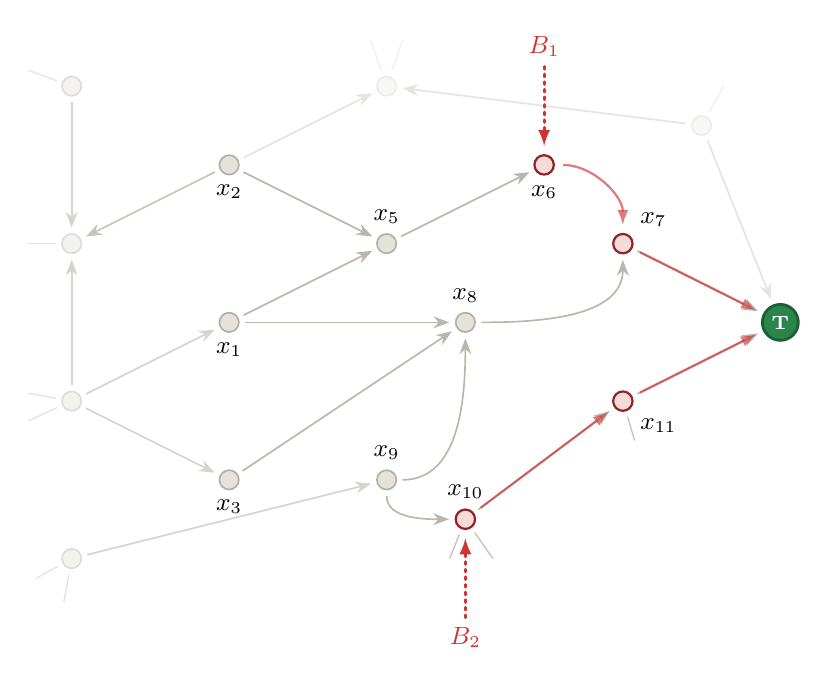
\begin{tikzpicture}[x=1cm, y=1cm]

  %% ── UBC nodes ─────────────────────────────────────────────────────────────
  %% Depth guide: ubc (closest to T / most visible)
  %%              ubc1 → ubc2 → ubc3 → ubc4 → ubcP (faintest / most distal)
  %%
  %% UBC 1
  \node[ubc1, label={[font=\small]below:$x_1$}]            (x1)  at (0.0,  0.0)  {};
  \node[ubc1, label={[font=\small]below:$x_2$}]            (x2)  at (0.0,  2.0)  {};
  \node[ubc1, label={[font=\small]below:$x_3$}]            (x3)  at (0.0, -2.0)  {};
  \node[ubc1, label={[font=\small]above:$x_5$}]            (x5)  at (2.0,  1.0)  {};
  \node[nodeB, label={[font=\small]below:$x_6$}]            (x6)  at (4.0,  2.0)  {};
  \node[nodeB, label={[font=\small]above right:$x_7$}]      (x7)  at (5.0,  1.0)  {};
  \node[ubc1, label={[font=\small]above:$x_8$}]            (x8)  at (3.0,  0.0)  {};
  \node[ubc1, label={[font=\small]above:$x_9$}]            (x9)  at (2.0, -2.0)  {};
  \node[nodeB, label={[font=\small]above:$x_{10}$}]         (x10) at (3.0, -2.5)  {};
  \node[nodeB, label={[font=\small]below right:$x_{11}$}]   (x11) at (5.0, -1.0) {};

  %% UBC 3
  \node[ubc3] (x12) at (-2.0, -3.0) {};
  \node[ubc3] (x13) at (-2.0, -1.0) {};
  \node[ubc3] (x14) at (-2.0,  1.0) {};
  \node[ubc3] (x15) at (-2.0,  3.0) {};

  %% UBC 4
  \node[ubc4] (x4)  at ( 2.0,  3.0) {};
  \node[ubc4] (x17) at ( 6.0,  2.5) {};

  %% ── Boarding / path nodes ─────────────────────────────────────────────────
  %% Replace the UBC-style node with ubc1 / nodeB / nodeAB at boarding points.
  %%
  \node[font=\small\bfseries, color=treatB] (nB1) at (4.0, 3.5)  {$B_1$};
  \node[font=\small\bfseries, color=treatB] (nB2) at (3.0, -4.0) {$B_2$};
  
  %% ── Target ────────────────────────────────────────────────────────────────
  \node[target] (T) at (7.0, 0) {T};

  %% ── UBC background edges ──────────────────────────────────────────────────
  \draw[ubc edge]  (x1) -- (x5);
  \draw[ubc edge]  (x1) -- (x8);
  \draw[ubc3 edge] (x2) -- (x4);
  \draw[ubc edge]  (x2) -- (x5);
  \draw[ubc edge]  (x3) -- (x8);
  \draw[ubc edge]  (x5) -- (x6);
  % \draw[ubc edge]  (x6) to[out=0, in=90] (x7);
  \draw[ubc edge]  (x8) to[out=0, in=-90] (x7);
  \draw[ubc edge]  (x9) to[out=0, in=-90] (x8);
  \draw[ubc edge]  (x9) to[out=-90, in=180] (x10);
  \draw[ubc edge]  (x10) -- (x11);
  \draw[ubc edge]  (x7) -- (T);
  \draw[ubc edge]  (x11) -- (T);
  \draw[ubc3 edge] (x17) -- (T);
  \draw[ubc3 edge] (x17) -- (x4);
  \draw[ubc1 edge] (x2) -- (x14);
  \draw[ubc2 edge] (x13) -- (x14);
  \draw[ubc2 edge] (x15) -- (x14);
  \draw[ubc2 edge] (x12) -- (x9);
  \draw[ubc2 edge] (x13) -- (x1);
  \draw[ubc2 edge] (x13) -- (x3);

  %% ── UBC stubs (outer nodes — graph continues beyond) ─────────────────────
  % left cluster (x12–x15): stubs going further left, diverging slightly
  \draw[ubc3 stub] (x15) -- +(-0.55,  0.20);
  \draw[ubc3 stub] (x14) -- +(-0.55,  0.00);
  \draw[ubc3 stub] (x13) -- +(-0.55,  0.10);
  \draw[ubc3 stub] (x13) -- +(-0.55, -0.25);
  \draw[ubc3 stub] (x12) -- +(-0.45, -0.25);
  \draw[ubc3 stub] (x12) -- +(-0.10, -0.55);
  % top nodes
  \draw[ubc4 stub] (x4)  -- +(-0.20,  0.58);
  \draw[ubc4 stub] (x4)  -- +( 0.20,  0.58);
  \draw[ubc4 stub] (x17) -- +( 0.28,  0.50);
  % bottom fringe
  \draw[ubc1 stub] (x10) -- +(-0.20, -0.50);
  \draw[ubc1 stub] (x10) -- +( 0.35, -0.50);
  \draw[ubc1 stub] (x11) -- +( 0.15, -0.50);

  %% ── Treatment path edges ──────────────────────────────────────────────────
  %% Draw A-only segments, then B-only segments, then shared in violet.
  %%
  \draw[treatB edge]    (x10) -- (x11);
  \draw[treatB edge]    (x11) -- (T);
  \draw[treatB edge]    (x6) to[out=0, in=90] (x7);
  \draw[treatB edge]    (x7) -- (T);
  
  %% ── Ingredient arrows ─────────────────────────────────────────────────────
  %% Arrow points FROM the ingredient TO the boarding node.
  %% Put the label at pos=0 (tail), offset away from the node.
  %%
  \draw[ingrB] (nB1) -- (x6);
  \draw[ingrB] (nB2) -- (x10);

\end{tikzpicture}
\end{document}